\documentclass[10pt,a4paper,ngerman, DIV=16]{scrartcl}
\usepackage{scrhack}
\usepackage{amsmath}
\usepackage{iftex}
\ifPDFTeX
	\usepackage[utf8]{inputenc}  % Deutsche Umlaute direkt eingeben
	\usepackage[T1]{fontenc}     % "Saubere" Schriften in der PDF
\else
	\ifXeTeX
		\usepackage{fontspec}
		\usepackage{unicode-math}
		\fontspec{DejaVu Serif}
		\setmainfont{DejaVu Serif} 
		\setsansfont{DejaVu Sans} 
		\setmonofont{DejaVu Sans Mono} 
		\setmathfont[math-style=TeX]{TeX Gyre DejaVu Math}
	\else
		\ifLuaTeX
			\usepackage{fontspec}
			\usepackage{luaotfload}
			\usepackage{luatextra}
%			\usepackage{lmodern}
			\usepackage{unicode-math}
			\fontspec{DejaVu Serif}
			\setmainfont{DejaVu Serif} 
			\setsansfont{DejaVu Sans} 
			\setmonofont{DejaVu Sans Mono} 
			\setmathfont[math-style=TeX]{TeX Gyre DejaVu Math}
		\fi
	\fi 				
\fi
\usepackage[ngerman]{babel}
\usepackage[ngerman]{translator}

\usepackage[babel, german=quotes]{csquotes}
\usepackage{gensymb}
\usepackage{textcomp}
\usepackage{hyperref}
\usepackage[]{varioref}
\usepackage[]{cleveref}
\usepackage{graphicx}
\usepackage{float}
\RedeclareSectionCommand[tocnumwidth=2em]{chapter}
\RedeclareSectionCommand[tocindent=3em,tocnumwidth=3.5em]{section}
\usepackage[]{todonotes}
\usepackage[toc, nopostdot, nonumberlist]{glossaries}
\makeglossaries

\usepackage{makeidx}
\makeindex

\setlength{\parindent} {0.0em}
\setlength{\parskip} {1.5ex plus0.5ex minus0.5ex}

\usepackage[backend=biber, %% Hilfsprogramm "biber" (statt "biblatex" oder "bibtex")
style=authoryear, %% Zitierstil (siehe Dokumentation)
natbib=true, %% Bereitstellen von natbib-kompatiblen Zitierkommandos
hyperref=true, %% hyperref-Paket verwenden, um Links zu erstellen
]{biblatex}
%\usepackage[backend=biber,style=alphabetic]{biblatex}
% die bib-Datei laden:
\addbibresource{Literatur.bib} %




\author{Thomas Kluth}
\title{Backwochende}
%\setcounter{tocdepth}{3}
%\setcounter{secnumdepth}{0}

\begin{document}
\maketitle
%\setcounter{tocdepth}{3}
\tableofcontents

\section{Seelachs mit Frühlingszwiebeln, Tomaten und Oliven}\label{sec:SeeLachs:TomatenOliven}\index{SeeLachs}\index{Fisch:SeeLachs}
\subsection*{Allgemeines}
\begin{tabular}{ll}
    Personen         &  4   \\
    Zubereitungszeit & 40 Minuten  \\
\end{tabular} 
\subsection*{Zutaten}
\begin{tabular}{r l}
    800 g & Seelachs                              \\
    400 g & Cocktailtomaten                       \\
    1 Bund & Frühlingszwiebeln                     \\
    5 EL & Olivenöl                              \\
    12 & getrocknete Tomaten in Öl (ca. 150 g) \\
    50 g & schwarze Oliven ohne Kern             \\
    2-3 & Kapern                                \\
    0,5 -1 TL & gemahlene Fenchelsaat                 \\
    0,5 TL & gemahlener Koriander                  \\
    0,5 TL & brauner Zucker                        \\
    & Salz und Pfeffer
\end{tabular}

Die Tomaten waschen und halbieren. Die Frühlingszwiebeln waschen, putzen und in grobe Stücke schneiden. Den Backofen auf 180 Grad (Ober-/Unterhitze) vorheizen.

Ein Backblech mit 2 Esslöffeln Olivenöl einfetten. Den Fisch, die Tomaten und Frühlingszwiebeln darauf verteilen. Die getrockneten Tomaten etwas abtropfen lassen, halbieren und mit den Oliven und Kapern auf dem Blech verteilen. Fenchelsaat, Koriander, Salz und Pfeffer auf den Fisch streuen. Alles mit dem restlichen Olivenöl beträufeln. Den braunen Zucker auf den Schnittflächen der Tomaten verteilen.

Im vorgeheizten Backofen etwa 20 bis 25 Minuten garen. Dazu schmeckt Baguette oder Ciabatta. Siehe \vref{sec:brot:Ciabatta:LM}.

\section{Backferment Weizen-Roggen-Vollkorn} \index{Brot!Weizen-Roggen}\index{Brot!Roggen}\index{Brot!Weizen}\index{Vollkorn!Brot}\index{Backferment!Brot}
\subsection*{Allgemeines}
\begin{tabular}{lrl}
    Gesamtzeit          & 16 --  24 & Stunden                       \\
    Vorteig erstellen   &        10 & Minuten                       \\
    Vorteig             &  12 -- 16 & Stunden                       \\
    Hauptteig erstellen &        10 & Minuten                       \\
    1. Gehzeit          &        50 & Minuten                       \\
    2. Gehzeit          &  30 -- 50 & Minuten                       \\
    Backzeit            &         1 & Stunden                       \\
    &           & \cite[Seite 66 ]{Pokorny2016}
\end{tabular} 
\subsection*{Zutaten}

\subsubsection*{Vorteig}
\begin{tabular}{lrr}
    Weizenvollkornmehl                  & 100 &  g \\
    Roggenvollkornmehl                  & 100 &  g \\
    lauwarmes Wasser (ca. 40 $^\circ$C) & 200 & ml \\
    Grundansatz                         &  10 &  g \\
    Backferment                         &   2 &  g
\end{tabular} 

Grundansatz mit Backferment in etwas Wasser auflösen, restliches Wasser zugeben und mit dem Vollkornmehl gründlich vermengen. Bedeckt bei ca. 24 $^{\circ} $C mindestens 12 Stunden stehen lassen. 

\subsubsection*{Hauptteig}
\begin{tabular}{lrr}
    Weizenvollkornmehl & 150 &  g \\
    Roggenvollkornmehl & 150 &  g \\
    sehr warmes Wasser (ca. 45 $^\circ$C) & 175 & ml \\
    Hefe   & 2-3          &   g \\
    Salz        & 10 & g \\
\end{tabular} 

\subsection*{Zubereitung}

\begin{enumerate}
    \item Zum Vorteig die gesalzenen Vollkornmehle hinzu gegeben und vermengen, Hefe in Wasser auflösen und nach und nach Wasser hinzugeben.
    \item Bedeckt 50 Minuten stehen lassen. Durchkneten, nach Belieben Körner (Sonnenblumen schmeckt gut, ca. 100~g) hinzugeben und in warme gefettete Backformen  (oder Garkörbchen) legen.
    \item Bedeckt weitere 40 Minuten stehen lassen. Backofen vorheizen ($ 220\;^{\circ} $C, Umluft $ 200\;^{\circ} $C) und Wasserschüssel einstellen. Teigestücke an der Oberfläche befeuchten und ca. eine Stunde backen.    
\end{enumerate}  


\section{Verdoppelung Lievito Madre: Dario}\index{Lievito Madre!Zubereitung}\label{sec:Lievito Madre}

\begin{enumerate}
    \item 100\;g Anstellgut wird 75\;g Wasser gemischt und dann ca. 10 Minuten ruhen lassen.  
    \item 100 g Weizen (Tippo  00) zugegeben und gut druchkneten
    \item Dann bei ca. 27 -- 29 Grad 3-4 Stunden reifen lassen.
    \item Braucht man mehr Lievito Madre, so kann man den Vorgang mehrmals wiederholen.
\end{enumerate}

\section{Verdoppelung Lievito Madre: Hartie}\index{Lievito Madre!Zubereitung}\label{sec:Lievito Madre:Hartie}

\begin{enumerate}
    \item 100\;g Anstellgut wird 50\;g Wasser gemischt und dann ca. 10 Minuten ruhen lassen.  
    \item 100 g Hartweizen  zugegeben und gut druchkneten
    \item Dann bei ca. 27 -- 29 Grad 3-5 Stunden reifen lassen.
    \item Braucht man mehr Lievito Madre, so kann man den Vorgang mehrmals wiederholen.
\end{enumerate}


\section{Ciabatta / Pain Paillasse} \label{sec:brot:Ciabatta:LM}  \index{Brot!Weizen}\index{Brot!Lievito Madre}\index{Ciabatta}

\subsection*{Allgemeines}
\begin{tabular}{lrl}
    Gesamtzeit          &   ca. 4.15 & Stunden \\
    Zutaten verrühren   &          8 & Minuten \\
    1. Teigruhe n       &         10 & Minuten \\
    Hauptteig erstellen &      10-12 & Minuten \\
    1. Gehzeit          &      ca. 3 & Stunden \\
    Formen              &          5 & Minuten \\
    2.Gehzeit           & 15 bzw. 45 & Minuten \\
    Backzeit            &     ca. 20 & Minuten
\end{tabular} 

\subsection*{Zutaten}

\begin{tabular}{r l}
    100 g & Lievito Madre TA 150 \\
    310 g & Wasser (kühl)        \\
    100 g & Hartweizenmehl       \\
    230 g & Weizenmehl  550er    \\
    8 g & Salz                 \\
    8 g & Olivenöl             \\
    4 g & Frischhefe
\end{tabular}

\subsection*{Zubereitung}
\begin{enumerate}
    \item Alle Zutaten in den Kneter geben. Mit dem Flachschlägerhaken  3 Minuten langsam rühren, bis alles zu einem Brei verrührt ist.
    \item 10 Minuten Pause.
    \item Dann auf Stufe 2-3 schalten und den Flachschlägerhaken so lange rühren lassen, bis sich der Teig komplett von der Schüssel löst. Das hat bei mir etwa 10-12 Minuten gedauert.
    \item Den Teig in eine Teigwanne geben und mindestens 2 1/2 bis 3 Stunden reifen lassen. Ggf. noch länger. Während der ersten 90 Minuten zwei mal dehnen und falten. Der Teig sollte sich gut verdreifacht haben vom Volumen und stark von Gasblasen durchzogen sein.
    \item Den Teig in eine Teigwanne geben und mindestens 2 1/2 bis 3 Stunden reifen lassen. Ggf. noch länger. Während der ersten 90 Minuten zwei mal dehnen und falten. Der Teig sollte sich gut verdreifacht haben vom Volumen und stark von Gasblasen durchzogen sein.
    \item Auf die gut bemehlte Arbeitsfläche kippen und die Rückseite bemehlen. Wenn die Teigwanne rechteckig war, von den kurzen Seiten her rasch und selbstsicher zwei Stücke abstechen. Mit den bemehlten Händen greifen und auf ein Backpapier legen. Dort dann mit raschen Handbewegungen die Teigstücke 3 – 4 mal (nicht zu oft) um sich selbst drehen, so dass die Wurzelform entsteht.
    \item Wenn es Ciabatta werden sollen, lediglich abstechen und auf das Backpapier befördern. Die Wurzelbrote noch etwa 15 Minuten entspannen lassen und dann sofort backen. Lässt man sie länger reifen, verwischen die Furchen zu stark. Ciabattateiglinge können noch gut und gerne 45 Minuten Stückgare vertragen, dann werden sie innen noch luftiger.
    \item Bei 250° in den gut vorgeheizten Ofen geben und sofort schwaden. Bei konstant 250° kräftig dunkel ausbacken,
\end{enumerate}




\section{Auffrischbrötchen Julchen}  \index{Brot!Weizen}\index{Brot!Lievito Madre}\index{Auffrischbrot! Brötchen Julchen}
\cite{sonjajulchen2022}
\subsection*{Allgemeines}
\begin{tabular}{lrl}
    Gesamtzeit          &   ca. 5.30 & Stunden \\
    Fermentolyseteig mischen   &   0.00        & Uhr \\
    Hauptteig zubereiten   &   0.30        & Uhr \\
    dehnen und falten   &   1.40        & Uhr \\
    dehnen und falte   &   2.40        & Uhr \\
    formen + Stückgare  &  3.50         & Uhr \\
    Backofen vorheizen &   4.30        & Uhr \\
    backen &   5.00        & Uhr \\
    aus dem Ofen holen  &   5.200        & Uhr \\
\end{tabular}

\subsection*{Zutaten}
\subsubsection*{Fermentolyseteig}
\begin{tabular}{r l}
    75 g & Lievito-Madre-Anstellgut + 25 g Wasser\\
    180 g & kalte Vollmilch (oder pflanzliche Alternative)\\
    120 g & kühles Wasser\\
    400 g & Weizenmehl Type 550\\
    50 g & Vollkornmehl nach Wahl\\
\end{tabular}\\
Alles kurz, aber gründlich mischen und für 20−30 Minuten abgedeckt quellen lassen.


\subsubsection*{Hauptteig}
\begin{tabular}{r l}
    & Fermentolyseteig                                      \\
    5 g & Frischhefe (oder 3 g bei kalter Übernachtgare         \\
    10 g & Honig oder Gerstenmalzextrakt (inaktives Flüssigmalz) \\
    11 g & Salz                                                  \\
    10 g & Butter (oder Olivenöl)                                \\
    20 g & Wasser nach Bedarf (Bassinage)                        \\
    & Roggenmehl zum Aufarbeiten (z. B. Type 610 oder 1150)
\end{tabular}\\


\subsection*{Zubereitung}
\begin{enumerate}
    \item [Teig] 
    \begin{itemize}
        \item Die Frischhefe und den Blütenhonig zum Fermentolyseteig geben und für 10 Minuten mit geringer Stufe kneten.
        \item Danach das Salz und die Butter zugeben und für 3–5 Minuten mit höherer Stufe auskneten, dabei bei Bedarf noch bis zu 20 g Wasser mit einkneten. )]
    \end{itemize}
    \item [Stockgare]
    \begin{itemize}
        \item Den Teig in einer leicht geölten Schüssel oder Teigwanne bei Raumtemperatur abgedeckt etwa 3 Stunden bis zur guten Verdopplung reifen lassen, dabei nach 1 und 2 Stunden schonend dehnen und falten (Coil fold).
        \item Variation kalte Stockgare: Für 90 Minuten bei Raumtemperatur (20−22 °C) anspringen lassen. Dabei nach jeweils 45 und 90 Minuten dehnen und falten. Danach für 12−14 Stunden bei 5 °C in den Kühlschrank geben. Anschließend für mindestens 1 Stunde akklimatisieren lassen.
    \end{itemize}
    \item [Formen]
    \begin{itemize}
        \item Den Teig auf der bemehlten Arbeitsfläche in neun Teile mit je etwa 95 g teilen.
        \item Die Teiglinge schonend rund wirken und dabei Roggenmehl in den Teigschluss einarbeiten, damit dieser während der Stückgare nicht verklebt.
        \item Danach mit dem Teigschluss nach unten in ein leicht bemehltes Bäckerleinen oder Geschirrtuch legen und den Stoff zwischen den Teiglingen etwas hochziehen, damit diese gestützt werden.
    \end{itemize}
    \item [\Gls{Stueckgare}]
    \begin{itemize}
        \item Die Teiglinge abgedeckt bei Raumtemperatur (20−22 °C) etwa 60–80 Minuten bis zur knappen Gare reifen lassen.
        \item Variation kalte Stückgare:  Die Teiglinge ohne Anspringen (gut eingepackt, z. B. mit XXL Gefrierbeuteln*) über Nacht 10–12 Stunden in den Kühlschrank bei 4–5 °C reifen lassen. (Die Kühlschranktemperatur bitte unbedingt nachmessen!) Danach ohne Akklimatisieren backen.
    \end{itemize}
    \item [Backen]
    \begin{itemize}
        \item Den Backofen rechtzeitig auf 240 °C Ober-/Unterhitze (220 °C Heißluft/Umluft) vorheizen, zusammen mit einem Backstahl oder Backstein.
        \item Die Teiglinge mit dem Teigschluss nach oben auf einem Bogen Backpapier oder Dauerbackfolie auf dem Einschießer verteilen.
        \item Anschließend einschießen und sofort schwaden. Insgesamt etwa 18−20 Minuten backen. Nach 10 Minuten den Dampf ablassen und die Temperatur auf 200 °C (180 °C Heißluft/Umluft) reduzieren.
        \item Anschließend sofort mit etwas Wasser einsprühen und auf einem Rost auskühlen lassen.
    \end{itemize}
\end{enumerate}

\section{Einfaches Auffrischbrot}  \index{Brot!Weizen}\index{Brot!Lievito Madre}\index{Auffrischbrot! Einfaches}
\begin{figure}
    \centering
    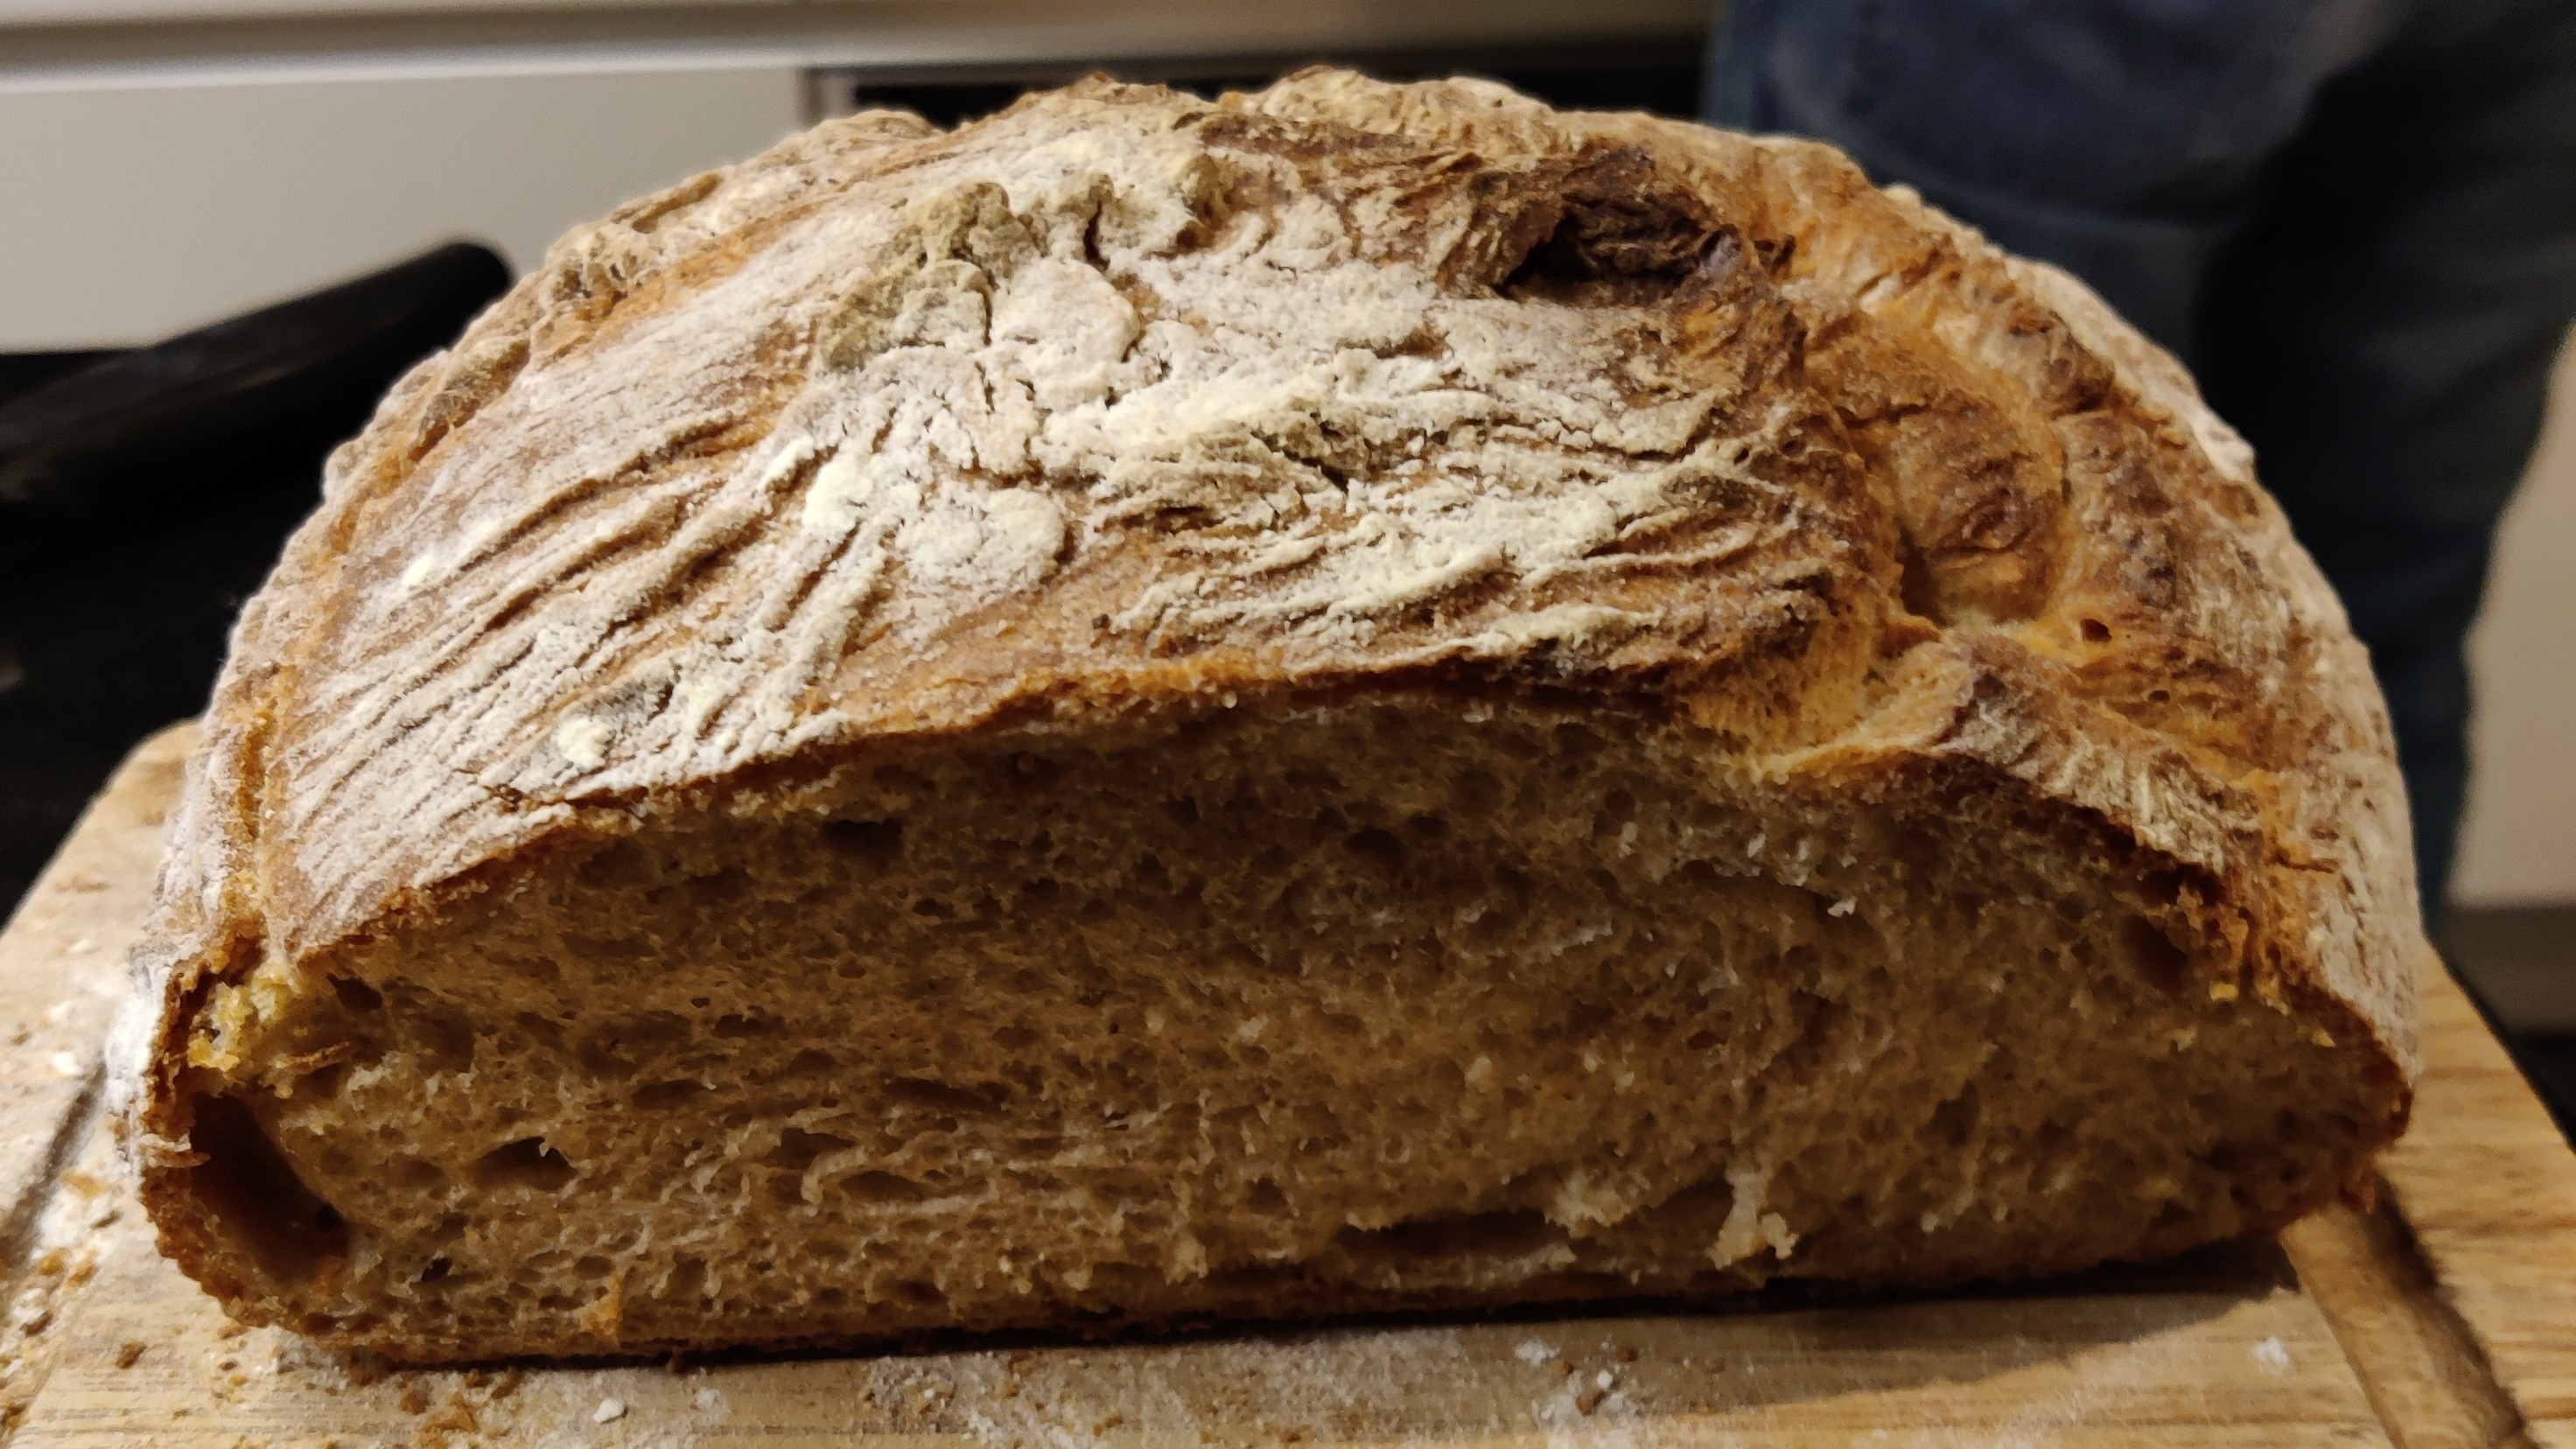
\includegraphics[width=0.7\linewidth]{Bilder/AuffrischbrotEinfach}
    \caption{Auffrischbrot Einfach}
    \label{fig:auffrischbroteinfach}
\end{figure}

\subsection*{Allgemeines}
\begin{tabular}{lrl}
    Gesamtzeit               &                ca. 5.30 & Stunden \\
    Fermentolyseteig mischen &                    0.00 & Uhr     \\
    Hauptteig zubereiten     &                    0.40 & Uhr     \\
    dehnen und falten        &                    1.40 & Uhr     \\
    dehnen und falte         &                    2.40 & Uhr     \\
    formen + Stückgare       &                    4.50 & Uhr     \\
    Backofen vorheizen       &                    5.50 & Uhr     \\
    backen                   &                    6.20 & Uhr     \\
    aus dem Ofen holen       &                    7.10 & Uhr     \\
    siehe                    & \cite{SonjaBauer2021} &
\end{tabular}

\subsection*{Zutaten}
\subsubsection*{\Gls{Fermentolyse}}
\begin{tabular}{r l}
    120 g & Lievito-Madre-Anstellgut + 30 g Wasser\\
    250 g & kühles Wasser\\
    250 g & Weizenmehl Type 550\\
    100 g & Weizenmehl Type 1050\\
    75  g & Vollkornmehl nach Wahl\\
\end{tabular}\\
Lievito Madre im Wasser auflösen, dann alles kurz, aber gründlich mischen und für 30 Minuten abgedeckt quellen lassen.


\subsubsection*{Hauptteig}
\begin{tabular}{r l}
    + & Fermentolyseteig                                      \\
    3 g & Frischhefe          \\
    10 g & Rübenkraut \\
    12 g & Salz                                                  \\
    10 g & Butter (oder Olivenöl)                                \\
    40 g & Wasser nach Bedarf (\Gls{Bassinage})                        \\
\end{tabular}\\


\subsection*{Zubereitung}
\begin{enumerate}
    \item [Teig] 
    \begin{itemize}
        \item Alle Zutaten (außer Salz + Bassinage) für 8–10 Minuten mit geringer Stufe kneten. Salz hinzufügen, für 3–5 Minuten mit höherer Stufe auskneten. Bei Bedarf noch bis zu
        40 g Wasser (Bassinage) mit einkneten.
    \end{itemize}
    \item [\Gls{Stockgare}]
    \begin{itemize}
        \item Den Teig in einer leicht geölten Schüssel oder Teigwanne bei Raumtemperatur abgedeckt etwa 3-4 Stunden bis zur guten Verdopplung reifen lassen, dabei nach 1 und 2 Stunden schonend dehnen und falten.
    \end{itemize}
    \item [\Gls{Ballengare}]
    \begin{itemize}
        \item Den Teig auf einer bemehlten Arbeitsfäche locker rund wirken und abgedeckt für 20 Minuten mit dem Schluss nach unten entspannen lassen. 
        \item Danach rund wirken und mit dem Schluss nach unten in ein bemehltes Gärkörbchen geben.
    \end{itemize}
    \item [\Gls{Stueckgare}]
    \begin{itemize}
        \item Abgedeckt für 90 Minuten bei Raumtemperatur (20−22 °C) reifen lassen.
    \end{itemize}
    \item [Backen]
    \begin{itemize}
        \item Den Backofen rechtzeitig auf 250 °C Ober-/Unterhitze  vorheizen, zusammen mit einem Backstahl oder Backstein.
        \item Den Teigling aus dem Gärkörbchen stürzen und einschießen. Sofort schwaden. 
        \item Nach 10 Minuten den Dampf ablassen und die Temperatur auf 210° C reduzieren. Weitere 40 Minuten backen.
    \end{itemize}
\end{enumerate}


\section{Jules Schwester}  \index{Brot!Weizen}\index{Brot!Lievito Madre}\index{Auffrischbrot! Jules Schwester}

\begin{figure}[H]
    \centering
    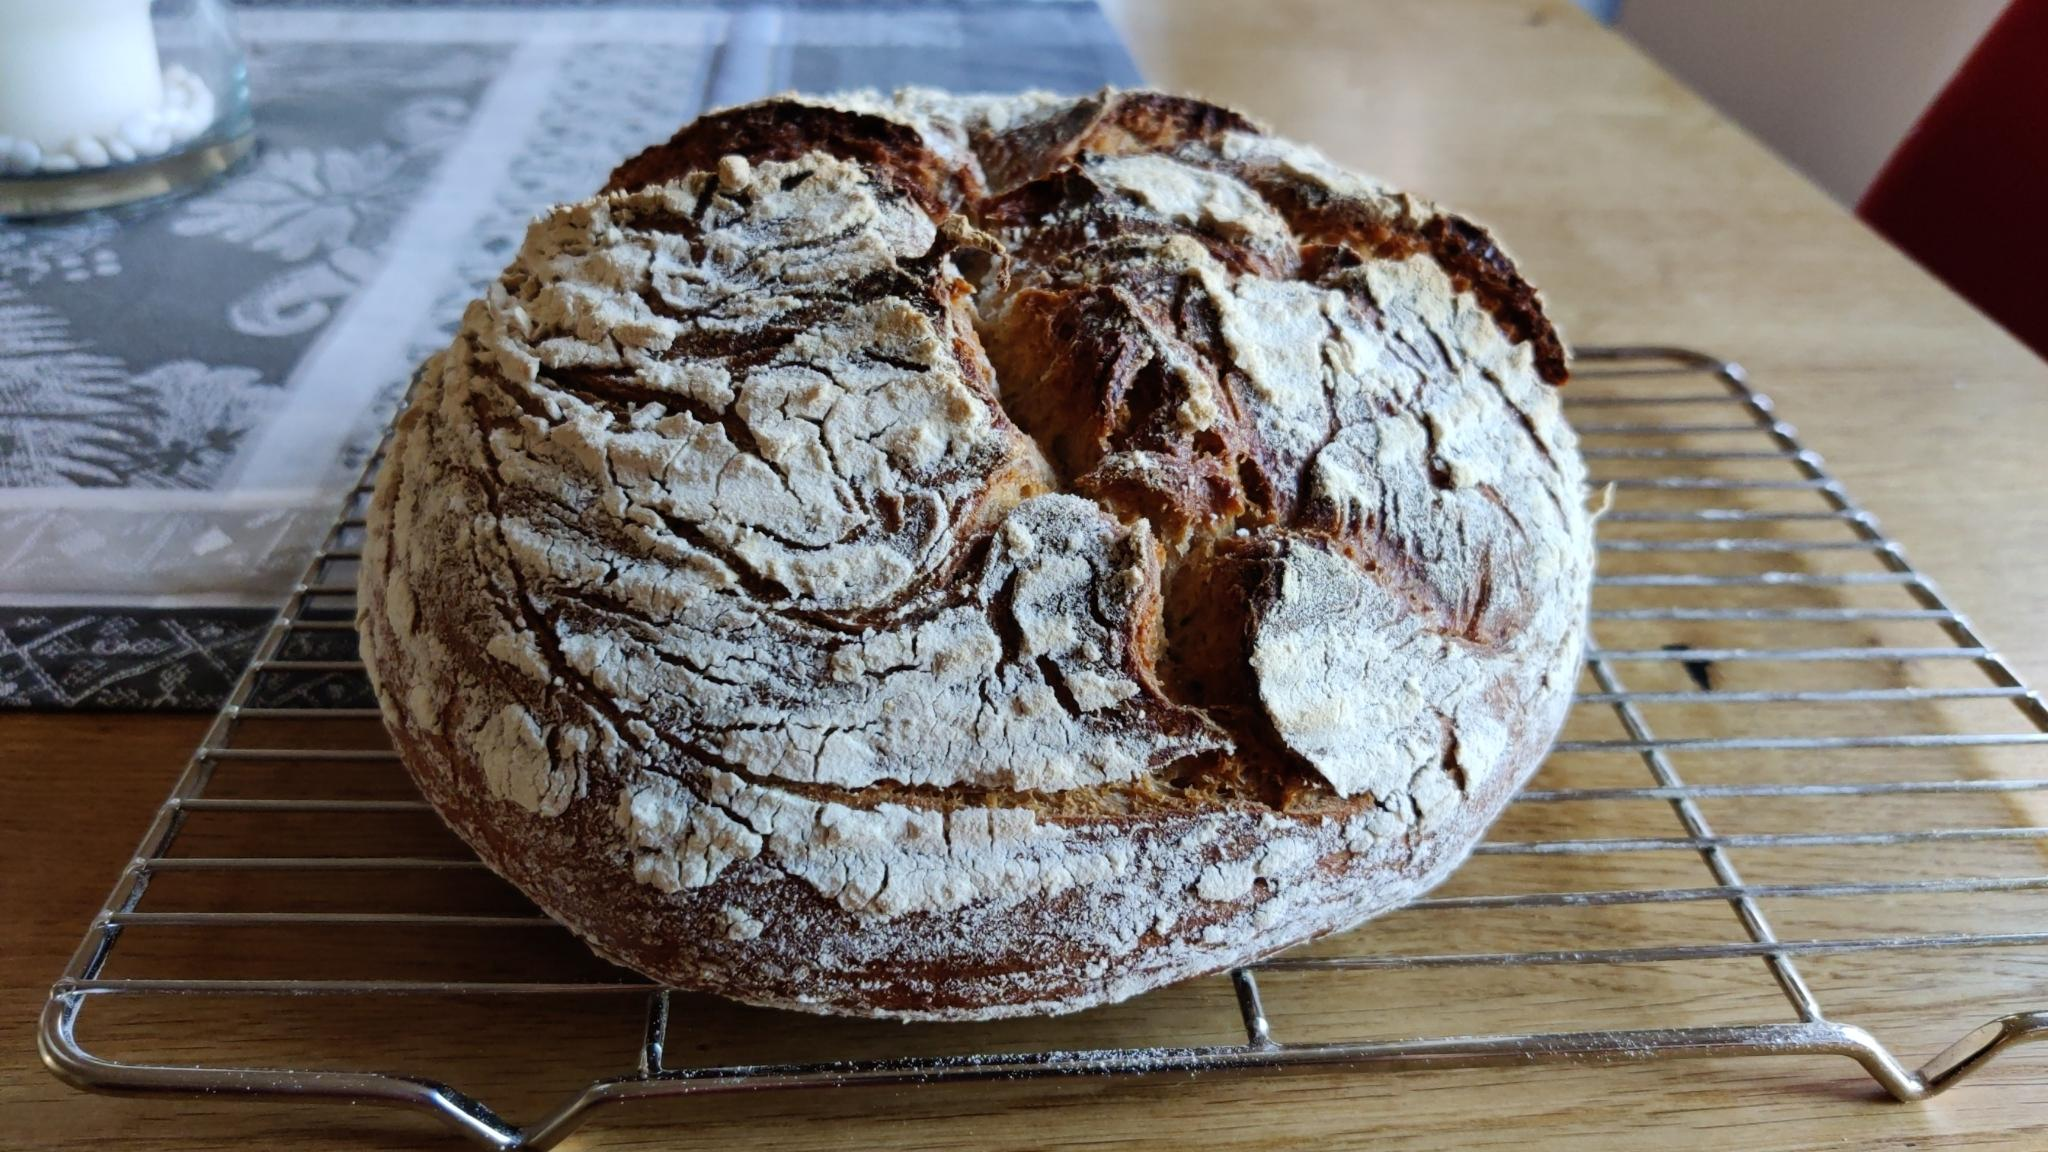
\includegraphics[width=0.7\linewidth]{Bilder/JulesSchwester}
    \caption{Jules Schwester}
    \label{fig:auffrischbrotJulesSchwester}
\end{figure}

\subsection*{Allgemeines}
\begin{tabular}{lrl}
    Gesamtzeit           &              ca. 5.30 & Stunden \\
    Brühstück            &               40 - 60 & Minuten \\
    Fermentolyseteig     &               30 - 40 & Minuten \\
    Hauptteig zubereiten &               11 - 15 & Minuten \\
    dehnen und falten    &                    60 & Minuten \\
    Stockgare            &               2,5  & Stunden \\
    formen + Stückgare   &                60- 80 & Minuten \\
    Backen               &                 50      & Minuten \\
    siehe                & \cite{SonjaBauer2021} &
\end{tabular}



\subsection*{Zubereitung}

\subsubsection*{\Gls{Bruehstueck}}
\begin{tabular}{r l}
    40 g & Altbrot geröstet\\
    120 g & heißer Kaffee\\
\end{tabular}\\

Kurz mischen und für mindestens 30–60 Minuten unbedeckt auf Raumtemperatur abkühlen lassen.

\subsubsection*{\Gls{Fermentolyse}}
\begin{tabular}{r l}
    150 g & Lievito-Madre-Anstellgut \\
    250 g & kühles Wasser\\
    200 g & Weizenmehl Type 550\\
    100 g & Weizenmehl Type 1050\\
\end{tabular}\\

Lievito Madre im Wasser auflösen, dann alles kurz, aber gründlich mischen und für 30 Minuten abgedeckt quellen lassen.


\subsubsection*{Hauptteig}
\begin{tabular}{r l}
    + & Fermentolyseteig                     \\
    + & Brühstück abgekühlt Fermentolyseteig \\
    5 g & Frischhefe                           \\
    10 g & Rübenkraut                           \\
    12 g & Salz                                 \\
    100 g & Roggenvollkornmehl                   \\
    30 g & Wasser nach Bedarf (\Gls{Bassinage})
\end{tabular}\\

Alle Zutaten (außer Salz + Bassinage) für 8–10 Minuten mit geringer Stufe kneten. Salz hinzufügen, für 3–5 Minuten mit höherer Stufe auskneten. Bei Bedarf noch bis zu 30 g Wasser (Bassinage) mit einkneten.


\subsubsection*{\Gls{Stockgare}}
Den Teig in einer leicht geölten Schüssel oder Teigwanne bei Raumtemperatur abgedeckt etwa 2,5 Stunden bis zur guten Verdopplung reifen lassen, dabei nach 1 dehnen und falten

\subsubsection*{\Gls{Ballengare}}
Den Teig auf einer bemehlten Arbeitsfäche locker rund wirken und abgedeckt für 20 Minuten mit dem Schluss nach unten entspannen lassen. 

\subsubsection*{\Gls{Stueckgare}}
Rund wirken und mit dem Schluss nach unten in ein bemehltes Gärkörbchen geben. Abgedeckt für 90 Minuten bei Raumtemperatur (20−22 °C) reifen lassen. 

\subsubsection*{Backen}
Den Backofen rechtzeitig auf 250 °C Ober-/Unterhitze  vorheizen, zusammen mit einem Backstahl oder Backstein.\\
Den Teigling aus dem Gärkörbchen stürzen und einschießen. Sofort schwaden. \\
Nach 10 Minuten den Dampf ablassen und die Temperatur auf 210° C reduzieren. Weitere 40 Minuten backen.


\section{Pizza-Teig}\label{sec:Pizza-Teig}\index{Pizza-Teig}

\subsection*{Allgemeines}
\begin{tabular}{lrl}
    Personen         &  6  &  \\
    Zubereitungszeit &  ? & Minuten \\
\end{tabular} 

\subsection*{Zutaten}
\begin{tabular}{lrl}
    10 &  g & frische Hefe \\
    600   & ml   & kaltes Wasser             \\
    1   & kg   & Mehl              \\
    8   & g & Salz           \\
\end{tabular} 


\subsection*{Zubereitung}

Es gibt die schnelle und die \glqq langsame\grqq\ Variante
\begin{enumerate}
    \item Hefe in 600 ml kaltes Wasser bröseln und 5 Minuten gut durchrühren.
    \item Mehl mit Salz zum Hefewasser geben und zu einem Teigkloß verarbeiten. Teig mit den Händen (Maschine funktioniert nicht wirklich) auf einer leicht bemehlten Oberfläche 10-15 Minuten geschmeidig kneten.
    
    {\large \textbf{Langsame Variante}}
    \begin{enumerate}
        \item Teig in eine große geölte Plastikdose geben und bis zu 8 Stunden in den Kühlschrank stellen. 
        \item 2 Stunden vor dem Backen den Teig auf die Arbeitsfläche gleiten lassen, 3 mal überfalten, wieder in die Dose geben.
        \item Abgedeckt nochmals 30 Minuten bei Zimmertemperatur gehen lassen. 
    \end{enumerate}
    
    {\large \textbf{Schnelle Variante}}
    \begin{enumerate}
        \item Teig Schüssel geben und luftdicht abschließen.
        \item Abgedeckt 1:30 Minuten bei Zimmertemperatur gehen lassen. 
    \end{enumerate}
    
    \item Teig auf der leicht bemehlten Arbeitsfläche zu einer Rolle formen, dabei nicht zu viel kneten. Rolle in 6 gleich große , ca. 250 g schwere Stücke teilen.
    \item Teigstücke zu Kugeln formen, mit ca. 10 cm Abstand in eine leicht bemehlte Form legen. Mit Mehl bestäuben und abgedeckt bei Zimmertemperatur eine Stunde gehen lassen.
    \item Teigkugeln jeweils mit den Händen auf der bemehlten Arbeitsfläche von innen nach außen zu dünnen runden oder ovalen Fladen drücken, den dabei entstehenden Rand nicht flachdrücken.
    \item Fladen jeweils auf ein Stück Backpapier geben, belegen und backen.
\end{enumerate}



\glsaddall

\newglossaryentry{Autolyse}{
    name={Autolyse},
    description={Siehe auch Nullteig. Die Autolyse bzw. der Autolyseteig wird vor der eigentlichen Teigzubereitung aus Mehl und Wasser oder an-
        deren Schüttflüssigkeiten gemischt und ruht meist abgedeckt für 20 bis 60 Minuten – manchmal auch bis zu 2 Stunden oder sogar über Nacht im Kühlschrank. Dabei verquellen Wasser, Stärke und Eiweißbestandteile aus dem Mehl. Während der Ruhezeit verkettet sich das Klebereiweiß (Gluten), und es bilden sich Glutenstränge (Teigstruktur). Dadurch kann die Knetzeit deutlich reduziert und einer zu starken Erwärmung beim Knetprozess vorgebeugt werden.
}}

\newglossaryentry{Backen}{
        name={Backen},
        description={Das Backen löst im Teig komplexe physikalische und chemische Prozesse aus. Je nach der Temperatur an der Teiglingsoberfläche und im Inneren des Teiglings beginnen unterschiedliche Vorgänge, bei denen sich Krume und Kruste bilden. Die jeweiligen Prozesse laufen nicht gleichmäßig im gesamten Teigling ab, sondern wandern von außen nach innen. Während zum Beispiel in den Randbereichen des Brotes schon alle Mikroorganismen durch die Hitze abgetötet sind, können sie im Inneren weiter für Ofentrieb sorgen.\\
        Quelle: \cite{PloetzblogLexikon2023}
        }}

\newglossaryentry{Ballengare}{
    name={Ballengare},
    description={Die sogenannte Ballengare oder Zwischengare dient als kurze Entspannungsphase für die Kleberstränge. Der Teig wird dabei zunächst locker vorgeformt (meinst rund) und ruht dann abgedeckt (z. B. mit einem Geschirrtuch) zwischen 5–20 Minuten. Dadurch lassen sich manche Teige besser formen oder reißen beim späteren Formen nicht. Anschließend folgt die endgültige Formgebung des Teiges.
}}

\newglossaryentry{Bassinage}{
    name={Bassinage},
    description={Verfahren, ein Teil des Schüttwassers im Knetprozess von Weizenteigen erst am Ende der Knetzeit schluckweise zuzugeben, wenn man bereits eine gute Kleberentwicklung erreicht hat. Dieses Verfahren wird insbesondere bei Teigen mit einem hohen Wassergehalt = hohe Teigausbeute genutzt.
}}

\newglossaryentry{Bruehstueck}{
    name={Brühstück},
    description={Das Brühstück gehört zur Gruppe der Nullteige innerhalb der Vorstufen. Es dient der Verquellung gröberer Brotbestandteile (z.B. Körner, Saaten, Schrote), um den Kaueindruck und die Frischhaltung zu verbessern (siehe auch Quellstück und Kochstück).\newline       
    Für ein Brühstück werden die festen Bestandteile im Verhältnis von ca. 1 : 1 bis 1 : 3 mit kochendem Wasser vermischt und mindestens 2-6 Stunden quellen gelassen. Eine noch optimalere und im Hobbybäckerbetrieb zeitlich passendere Variante ist das Verquellen über 8-12 Stunden bei 6-8°C im Kühlschrank (nachdem das Brühstück ausgekühlt ist). Um enzymatischen Abbau und Fremdgärung zu verhindern, kann die Salzmenge des Hauptteiges mit in das Brühstück eingerührt werden.\newline
    Würden die groben Bestandteile nicht verquollen, würde der Wassergehalt im Teig sinken und der Teig durch Nachquellung zunehmend fester und trockener werden. Üblicherweise sollte die im Brühstück zu verquellende Schrotmenge nicht mehr als 30-50\% der Gesamtmenge der Getreideerzeugnisse ausmachen, da durch das heiße Wasser bereits Stärke verkleistert und dem enzymatischen Abbau stärker ausgesetzt ist.\newline 
    Neben Schrot kann z.B. auch getrocknetes und gemahlenes Brot überbrüht werden. Dieses Altbrot bindet etwa die dreifache Menge seines Eigengewichtes an Wasser.\newline
    Quelle: \cite{PloetzblogLexikon2023} 
}}

\newglossaryentry{DehnenUndFalten}{
        name={Dehnen und Falten},
        description={Das Dehnen und Falten von Teig ist ein Vorgang, bei dem weizendominierten Teigen durch mehrfache Dehnung und Faltung mehr Struktur verliehen wird. Das Klebergerüst wird damit schonend entwickelt. Das Gashaltevermögen steigt. Außerdem dient es der Entgasung und Sauerstoffzufuhr, der Homogenisierung der Teigtemperatur und damit der Unterstützung der mikrobiellen Aktivität.\newline
        Quelle: \cite{PloetzblogLexikon2023} 
        }}

\newglossaryentry{Fermentolyse}{
    name={Fermentolyse},
    description={Das Pendant zur \Gls{Autolyse}. Im Gegensatz dazu ist aber bereits ein Triebmittel (Sauer teig/Vor teig) enthalten. Dadurch verkürzt sich das Vorquellen deutlich auf maximal 20 bis 40 Minuten. Dabei verquellen Wasser, Stärke und Eiweißbestandteile aus dem Mehl. Während der Ruhezeit verkettet sich das Klebereiweiß (Gluten), und es bilden sich Glutenstränge (Teigstruktur). Dadurch kann die Knetzeit deutlich reduziert und einer zu starken Erwärmung beim Knetprozess vorgebeugt werden.
}}


\newglossaryentry{Formen}{
    name={Formen},
    description={Nach der Stockgare und vor der nachfolgenden Stückgare wird der Teig geformt. Der Teig kann rund geformt werden (rundwirken), länglich (langwirken) oder auch in allerlei andere Formen gebracht werden. Dies erfolgt überwiegend auf der bemehlten und selten auf der mit Wasser benetzten Arbeitsfläche.\\
    Ziel ist in aller Regel dabei, dass der Teig nicht nur in Form gebracht wird, sondern an der Teigoberfläche auch eine gewisse Spannung aufbaut. Der Teig sollte dabei aber nur so weit gestrafft werden, dass er nicht reißt.       
}}


\newglossaryentry{Hauptteig}{
        name={Hauptteig},
        description={Der Teig, in dem alle Bestandteile des Brotes enthalten sind.
        }}

\newglossaryentry{LievitoMadre}{
    name={Lievito Madre},
    description={Lievito Madre ist Italiens Antwort auf den traditionellen Sauerteig. Mit seiner festen Konsistenz und dem milden Geschmack ist er ein unverzichtbares Element in der italienischen Brotkultur. Ein Lievito Madre ist ein spezieller italienischer Weizensauerteig, der fest geführt wird. Er ist mild und triebstark und auch für süße Backwaren geeignet.         
}}

\newglossaryentry{Quellstueck}{
    name={Quellstück},
    description={Ein Quellstück ist eine wichtige Komponente beim Brot backen, insbesondere wenn das Rezept gröbere oder trockenere Zutaten wie Altbrot, Samen, Schrot oder Trockenfrüchte enthält. Dieser sogenannte Nullteig oder Vorstufe hilft dabei, diese trockenen Zutaten vorzuquellen, indem sie in einem Verhältnis von etwa 1:1 bis 1:2 mit kühlem oder lauwarmem Wasser übergossen werden.
}}

\newglossaryentry{Sauerteig}{
        name={Sauerteig},
        description={In einem Sauerteig entwickeln sich homofermentative (milchsäurebildende) und
        heterofermentative (essigsäurebildende) Milchsäurebakterien (letztere werden oftmals fälschlicherweise als Essigsäurebakterien bezeichnet), außerdem Hefen. 
        Die heterofermentativen Bakterien erzeugen außerdem Kohlenstoffdioxid, das gemeinsam mit dem Kohlenstoffdioxid der alkoholischen Hefegärung das Gärgas bildet und für den Trieb sorgt.
        }}

\newglossaryentry{Stueckgare}{
    name={Stückgare},
    description={
        Die letzte Reifezeit des geformten Teiges vor dem Backen. Die Stückgare er folgt entweder mit Schluss nach oben oder nach unten in einem Gärkörbchen, Bäckerleinen oder in einer Backform.
        Die Stückgare kann je nach Rezept bei Raumtemperatur, an einem
        warmen Ort oder auch kalt erfolgen.
}}
\newglossaryentry{Stockgare}{
    name={Stockgare},
    description={Zeit die man dem Teig nach dem Kneten lässt um sich zu entwickeln. Weiche Weizenteige werden oft während der Stockgare gedehnt und gefaltet um die Teigstruktur zu verbessern. Zur Stockgare wird der Teig in einer Schüssel oder Wanne luftdicht abgedeckt damit er nicht austrocknet
}}

\newglossaryentry{Vorheizen}{
        name={Vorheizen},
        description={Der Ofen sollte bei Ober/Unterhitze ausreichend lange vorgeheizt werden, um das perfekte Brot zu backen. Umluft eignet sich weniger gut, da diese Einstellung die Oberfläche des Brotes zu schnell austrocknen würde.
        }}

\newglossaryentry{Zwischengare}{
    name={Zwischengare},
    description={Die Zwischengare ist eine sehr kurze (ca. 5 – 30 Minuten) Ruhephase zwischen Arbeitsvorgängen. Häufig wird die Zwischengare genutzt, um die Kleberstränge rundgewirkter Teiglinge kurz entspannen zu lassen. Andernfalls würde die Teigoberfläche beim weiteren Wirken reißen. \cite{PloetzblogLexikon2023}
}}




%\newglossaryentry{ }{
    %    name={},
    %    description={
        %}}


%
%
%
%Beschreibung:
%Das Brühstück gehört zur Gruppe der Nullteige innerhalb der Vorstufen. Es dient der Verquellung gröberer Brotbestandteile (z.B. Körner, Saaten, Schrote), um den Kaueindruck und die Frischhaltung zu verbessern (siehe auch Quellstück und Kochstück).
%
%Für ein Brühstück werden die festen Bestandteile im Verhältnis von ca. 1 : 1 bis 1 : 3 mit kochendem Wasser vermischt und mindestens 2-6 Stunden quellen gelassen. Eine noch optimalere und im Hobbybäckerbetrieb zeitlich passendere Variante ist das Verquellen über 8-12 Stunden bei 6-8°C im Kühlschrank (nachdem das Brühstück ausgekühlt ist). Um enzymatischen Abbau und Fremdgärung zu verhindern, kann die Salzmenge des Hauptteiges mit in das Brühstück eingerührt werden.
%
%Würden die groben Bestandteile nicht verquollen, würde der Wassergehalt im Teig sinken und der Teig durch Nachquellung zunehmend fester und trockener werden. Üblicherweise sollte die im Brühstück zu verquellende Schrotmenge nicht mehr als 30-50% der Gesamtmenge der Getreideerzeugnisse ausmachen, da durch das heiße Wasser bereits Stärke verkleistert und dem enzymatischen Abbau stärker ausgesetzt ist.
%
%Neben Schrot kann z.B. auch getrocknetes und gemahlenes Brot überbrüht werden. Dieses Altbrot bindet etwa die dreifache Menge seines Eigengewichtes an Wasser.
%
%Quellen:
%Steffen, Lutz Geißler
%/home/thomas/Sandbox/Privat/Privat/Text/Kochbuch/Glossar.tex
%A
%
%Anstellgut (ASG) : Als Anstellgut bezeichnet man die Sauerteigkultur, die man zum Ansetzen eines neuen Sauerteigs benutzt. Ich lagere meine Sauerteigkultur = Anstellgut im Marmeladenglas im Kühlschrank für bis zu 3 Wochen. Dann muss die Kultur aufgefrischt werden, d.h. 50 g Mehl/50 g Wasser/10 g alte Kultur = Anstellgut für ca. 16-20 h von 30° C auf Raumtemperatur fallend stehen lassen, danach im Kühlschrank lagern. Grundsätzlich kann man einen Sauerteig durch Auffrischen mit einer anderen Mehlsorte umzüchten, also z.B. von Roggen- nach Weizensauerteig. Teilweise wird das Anstellgut auch als Starter bezeichnet.
%
%Auffrischen: Als Auffrischen bezeichnet der Bäcker das Füttern der Sauerteigkultur mit frischem Mehl und Wasser, damit die Mikroorganismen frische Nahrung bekommen und sich wieder vermehren können. Übliche Verhältnisse zum Auffrischen von weichem Sauerteig ist ein Verhältnis 1:5:5 oder 1:10:10 von Anstellgut/Wasser/Mehl.
%
%Autolyse: Als Autolyse bezeichnet man das Quellenlassen von Mehl mit Wasser für 20-60 min ohne die Zugabe von Salz. Dabei quellen die Stärke und die Eiweiße im Mehl auf, was die Backeigenschaften verbessert und das Kneten beschleunigt.
%B
%
%Bassinage: Verfahren, ein Teil des Schüttwassers im Knetprozess von Weizenteigen erst am Ende der Knetzeit schluckweise zuzugeben, wenn man bereits eine gute Kleberentwicklung erreicht hat. Dieses Verfahren wird insbesondere bei Teigen mit einem hohen Wassergehalt = hohe Teigausbeute genutzt.
%D
%
%Dehnen und Falten (oft auch  “stretch and fold” oder s+f genannt)
%Weiche Weizenteige können über das wiederholte dehnen und falten schonend eine gute Struktur bekommen. Dazu wird, vorzugsweise  in einer geölten Wanne oder Schüssel, mit den feuchten Händen eine Seite des Teigs nach oben gezogen und dann über den Teig gefaltet , diesen Vorgang wiederholt man  auf den anderen 3 Seiten. Nach 20 -30 min kann man dann eine weitere Runde starten. Man merkt dabei, dass der Teig wesentlich mehr Struktur bekommt und straffer wird.
%E
%
%Einschießer/Einschießen
%Als Einschießen bezeichnet man den Vorgang den Teigling  mit einem Schieber oder Einschießer in den  Ofen zu bringen. Als Hobbybäcker benutzt man dafür meist ein passendes Brett und verwendet als Trennmittel Gries, feinen Schrot oder einfach Backpapier.
%
%Entgasen/Ausstoßen
%Wenn ein Teig nach der Stockgare gut aufgegangen ist, drückt man ihn mit der flachen Hand oder der Faust auf der Arbeitsfläche platt und sorgt damit dafür, dass sich große Gärblasen verteilen und auch ein Austausch von Kohlendioxid gegen Luftsauerstoff stattfindet was die weitere Entwicklung der Hefen fördert.
%F
%
%Fenstertest: Der Fenstertest dient zur Beurteilung der Kleberentwicklung eines weizenlastigen Teiges. Dazu zieht man den gekneteten Teig zwischen den feuchten Fingern so dünn, dass Licht durchscheint. Reißt der Teig davor ist er noch nicht ausreichend geknetet.
%
%Fingertest: Mit dem Fingertest prüft man die Gare eines Teiglings während der Stückgare: Dazu drückt man leicht mit dem Finger auf den Teigling und kann mit etwas Erfahrung die folgenden Garezustände unterscheiden:
%
%Untergare: Abdruck springt schnell und komplett wieder zurück
%knappe Gare: Abdruck geht langsam und fast  komplett zurück
%Volle Gare: Abdruck geht nur noch wenig zurück es bleibt eine leichte Delle
%Übergare: Abdruck bleibt unverändert oder Teigling fällt sogar zusammen
%
%G
%
%Glutenentwicklung: (Kleberentwicklung) Beim Kneten des Teigs vernetzt sich das Gluten (Kleber) immer stärker, um ein großvolumiges Brot zu erhalten ist eine gute Glutenentwicklung notwendig, diese kann durch den sog. Fenstertest überprüft werden.
%H
%
%Hefe: Hefe ist neben Sauerteig das wichtigste Triebmittel in allen Brotteigen. Man kann Trocken- oder Frischhefe einsetzen. Alle Angaben in meinen Rezepten beziehen sich auf Frischhefe.
%Umrechnungsregel: Trockenhefe in Frischhefe: 1 g Trockenhefe entspricht 3 g Frischhefe.
%Als Hilfe für das Portionieren kleiner Hefemengen gibt es eine sog. Hefeschablone, auch käuflich bei der Draxmühle zu erwerben.
%L
%
%Lievito Madre (LM): LM ist ein sehr milder und triebstarker Weizensauerteig italienischem Ursprungs. Er wird oft für helle Brote, Brötchen und auch für Pannetone verwendet. LM wird recht fest, mit einer Teigausbeute von 150 geführt, d.h. auf 100 g Mehl 50 g Wasser und führt zu einem starken Ofentrieb.
%
%Aufgefrischt wird LM normalerweise so: 1 Teil alter LM, 1 Teil Weizenmehl, 0,5 Teile Wasser (35 -40°C) zu einem festen Teig verkneten, kreuzwesie einschneiden und abgedeckt 4 h bei 30°C gehen lassen.  Dabei soltle er sich mindestens verdoppeln. Dann ist er zum Backen bereit. Nicht vergessen etwas LM abzuzweigen und als “Starterkultur” im Kühlschrank aufbewahren.
%
%Langwirken: Als Langwirken bezeichnet man das Formen eines länglichen Brotlaibs. Man startet immer in dem man den Teig rundwirkt (siehe unten) und ihn. dann nach kurzer Entspannungspause in eine längliche Form bringt. Dafür gibt es diverse Techniken, z.B. hier im Video erklärt.
%P
%
%Poolish: Flüssiger Weizenvortieg mit Hefe: Weizenmehl wird 1:1 mit Wasser gemischt und mit wenig Hefe  (0,2-0,3 %) versetzt und 12-14 h bei Raumtemperatur oder im Kühlschrank stehen lassen.
%R
%
%Rundschleifen: Nennt der Bäcker den Vorgang zum Formen runder Brötchen, es gibt diverse Filmchen dazu bei YouTube
%
%Rundwirken:  So nennet man den Vorgang aus einem Teig einen runden Laib zu formen und dabei im Teig Spannung aufzubauen.  Am besten schaut mich das in einem Video auf YouTube an
%S
%
%Schluß: Die Seite eines Teiglings auf der der Teig eingefaltet wird um Spannung im Teigling zu erzeugen, wird als Schluß bezeichnet. Backt man ein Brot oder Brötchen mit dem Schluß nach oben, reisst die Oberfläche rustikal auf und es muss nicht eingeschnitten werden.
%
%Schwaden: Bäckerdeutsch für  Dampf, der im Ofen erzeugt wird, dies ist insbesondere in der ersten Backphase wichtig damit, ein guter Ofentrieb und eine schöne rösche Kruste erhalten wird. Später wird der Dampf meist abgelassen, damit die Kruste kross wird.
%
%Stippen: So nennt der Bäcker den Vorgang in die Oberfläche eines Teiglinge vor dem Backen kleine Löcher zu machen, dafür gibt es spezielle Stippwalzen/Stipproller/Teigigel oder man behilft sich z.B. mit einem Schaschlikspieß oder ähnlichem. Die dient dazu bei einem fast vollgaren Brot das aufreißen der Kruste zu verhindern.
%
%t.
%
%Stückgare: Zeit in dem sich der Teigling nach dem Formen entwickelt und die richtige Gare vor dem Backen erreicht. Wichtig ist es die Teiglinge mit einem Küchentuch und Folie abzudecken, damit sie nicht austrocknen.
%T
%
%Teigausbeute (TA): Die Teigausbeute gibt das Verhältnis von Mehl zu Flüssigkeit im Teig an, eine hohe Teigausbeute bedeutet, dass viel Flüssigkeit im Teig vorhanden ist. Berechnet wird sie folgendermaßen: Teigausbeute = Flüssigkeitsmenge/Mehlmenge*100+100,
%also z.B. 650g  Wasser /1000g Mehl ergeben eine TA von 165.
%W
%
%Wirken:  Mit dem Begriff “wirken” bezeichnet der Bäcker das in Form bringen von Teiglingen mit speziellen Techniken, welche Spannung im Teigling erzeugen und für die Krumenstruktur und das Volumen des Brots eine sehr wichtige Rolle spielen. Man unterscheidet insbesondere das Rundwirken von runden Laiben und das Langwirken von länglichen Laiben.



\listoffigures
\printglossary[title=Glossar]
\printindex
\printbibliography 
%\listoftodos
\end{document}